\documentclass[aspectratio=169]{beamer}
\usepackage[utf8]{inputenc}
\usepackage[T1]{fontenc}
\usepackage{kotex}
\usepackage{graphicx}
\usepackage{booktabs}
\usepackage{xcolor}

\definecolor{MonoBlack}{HTML}{111111}
\definecolor{MonoDark}{HTML}{2F2F2F}
\definecolor{MonoMid}{HTML}{6E6E6E}
\definecolor{MonoLight}{HTML}{E9E9E9}
\definecolor{MonoWhite}{HTML}{FFFFFF}

\setbeamertemplate{navigation symbols}{}
\setbeamertemplate{items}[circle]
\setbeamertemplate{frametitle}{
    \vspace{0.4em}
    \insertframetitle\par
    \vspace{0.35em}
    {\color{MonoLight}\rule{\linewidth}{0.6pt}}
}

\setbeamercolor{normal text}{fg=MonoBlack,bg=MonoWhite}
\setbeamercolor{title}{fg=MonoBlack}
\setbeamercolor{subtitle}{fg=MonoDark}
\setbeamercolor{author}{fg=MonoDark}
\setbeamercolor{date}{fg=MonoMid}
\setbeamercolor{frametitle}{fg=MonoBlack,bg=MonoWhite}
\setbeamercolor{structure}{fg=MonoBlack}
\setbeamercolor{item}{fg=MonoBlack}
\setbeamercolor{section in toc}{fg=MonoBlack}
\setbeamercolor{section number projected}{fg=MonoWhite,bg=MonoBlack}
\setbeamercolor{block title}{fg=MonoWhite,bg=MonoBlack}
\setbeamercolor{block body}{fg=MonoBlack,bg=MonoLight}

\setbeamerfont{title}{series=\bfseries,size=\LARGE}
\setbeamerfont{subtitle}{size=\large}
\setbeamerfont{frametitle}{series=\bfseries,size=\Large}
\setbeamerfont{author}{size=\normalsize}
\setbeamerfont{date}{size=\small}

\title{A7608 컴퓨터비전 Chapter 3.2}
\subtitle{비지도학습}
\author{Draft}
\date{2026-03-29}

\begin{document}

\frame{\titlepage}

\begin{frame}{발표 흐름}
\tableofcontents
\end{frame}

\section{개요}
\begin{frame}{비지도학습}
\begin{itemize}
    \item 레이블 없이 데이터 구조를 찾는 학습 방식
    \item 대표 작업: 군집화, 차원 축소, 밀도 기반 탐색
    \item Chapter 3.2 실습은 K-means와 PCA 기반 시각화에 초점
\end{itemize}
\end{frame}

\begin{frame}{세미나 진행 방식}
\begin{block}{이번 발표의 흐름}
\begin{itemize}
    \item 교재에서 개념을 먼저 설명한다.
    \item 같은 내용을 \texttt{python\_3장.ipynb}의 해당 셀에서 바로 확인한다.
    \item 발표 중간에 ``자, 여기 실습해보아요'' 흐름으로 노트북을 실행한다.
\end{itemize}
\end{block}
\begin{block}{노트북 기준}
\begin{itemize}
    \item K-means: 셀 \texttt{34--39}
    \item PCA + DBSCAN: 셀 \texttt{40--47}
\end{itemize}
\end{block}
\end{frame}

\section{K-means}
\begin{frame}{K-means 핵심 개념}
\begin{itemize}
    \item 목표는 비슷한 데이터끼리 같은 군집으로 묶는 것이다.
    \item K-means는 군집 개수 \(k\)를 먼저 정하고, 각 군집의 중심을 반복적으로 갱신한다.
    \item 결과 해석의 핵심은 ``몇 개의 군집으로 보는 것이 자연스러운가''이다.
    \item 실습에서는 엘보우 곡선을 사용해 \(k\)를 고르는 감각을 만든다.
\end{itemize}
\end{frame}

\begin{frame}{K-means Notebook 흐름}
\begin{block}{교재 설명 뒤 바로 확인할 셀}
\begin{itemize}
    \item 셀 \texttt{34}: K-means 섹션 시작
    \item 셀 \texttt{35--36}: 데이터 로드와 기본 확인
    \item 셀 \texttt{37}: \texttt{Channel}, \texttt{Region} 원-핫 인코딩
    \item 셀 \texttt{38}: \texttt{MinMaxScaler}로 정규화
    \item 셀 \texttt{39}: \(k=1\)부터 \(14\)까지 inertia 계산 후 엘보우 곡선 그림
\end{itemize}
\end{block}
\begin{block}{발표 멘트 포인트}
\begin{itemize}
    \item 범주형 변수는 숫자로 바꾸지 않으면 거리 계산이 왜곡된다.
    \item 스케일이 큰 특성이 중심 업데이트를 지배하지 않도록 정규화가 필요하다.
    \item 여기서부터는 책 설명을 멈추고 노트북으로 넘어가 바로 돌려볼 수 있다.
\end{itemize}
\end{block}
\end{frame}

\begin{frame}{K-means 실습 결과 해석}
\begin{itemize}
    \item 데이터: \texttt{sales data.csv}
    \item 전처리: 범주형 원-핫 인코딩, 수치형 정규화
    \item 핵심 메시지: 관성(inertia) 감소 곡선이 급하게 꺾이는 구간을 찾는다.
    \item 발표 중에는 ``왜 \(k\)가 커질수록 inertia는 항상 감소하는가''를 먼저 짚어주면 좋다.
\end{itemize}
\begin{center}
    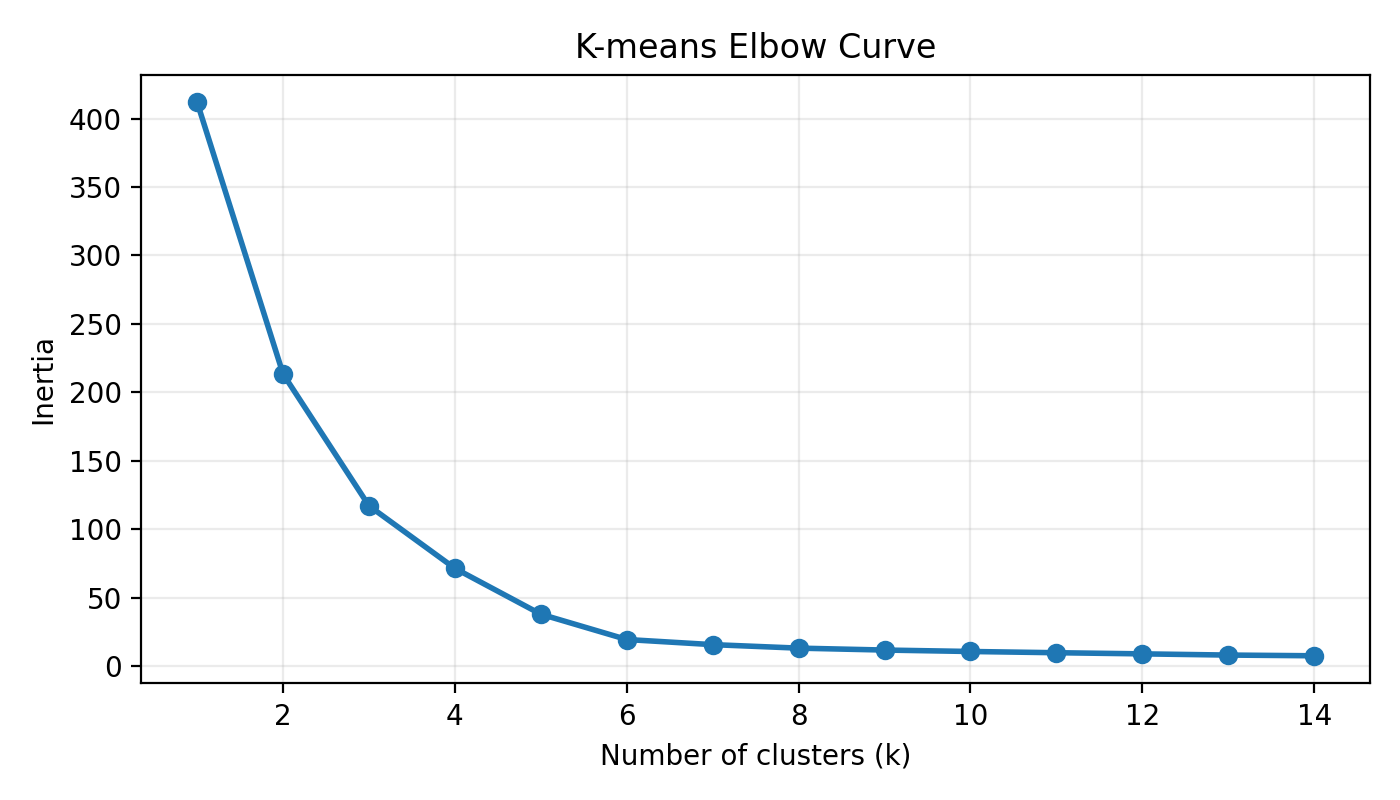
\includegraphics[width=0.72\linewidth]{figures/kmeans_elbow.png}
\end{center}
\end{frame}

\begin{frame}{실습 전환 멘트: K-means}
\begin{block}{슬라이드에서 노트북으로 넘어가는 순간}
\small
``여기까지가 교재가 말하는 K-means의 개념입니다. 이제 같은 내용을 노트북 셀 34번부터 39번까지 직접 보면서, 범주형 인코딩과 정규화가 어떻게 들어가고 엘보우 곡선이 어떻게 만들어지는지 확인해보겠습니다.''
\end{block}
\begin{block}{실행할 것}
\begin{itemize}
    \item \texttt{python\_3장.ipynb} 셀 \texttt{34--39}
    \item 결과 그림: \texttt{slides/figures/kmeans\_elbow.png}
\end{itemize}
\end{block}
\end{frame}

\section{PCA + DBSCAN}
\begin{frame}{PCA가 필요한 이유}
\begin{itemize}
    \item 고차원 데이터는 그대로는 눈으로 군집 구조를 보기 어렵다.
    \item PCA는 분산이 큰 방향을 기준으로 축을 다시 잡아 저차원 표현을 만든다.
    \item 실습에서는 여러 소비 패턴 특성을 2차원으로 줄여 시각화 가능한 공간으로 바꾼다.
    \item 즉, PCA는 군집 알고리즘 자체라기보다 ``구조를 보이게 만드는 전처리'' 역할이다.
\end{itemize}
\end{frame}

\begin{frame}{PCA + DBSCAN Notebook 흐름}
\begin{block}{교재 설명 뒤 바로 확인할 셀}
\begin{itemize}
    \item 셀 \texttt{40}: PCA 섹션 시작
    \item 셀 \texttt{41--42}: 데이터 로드, \texttt{CUST\_ID} 제거, 결측치 처리
    \item 셀 \texttt{43}: 표준화, 정규화, PCA 2차원 투영
    \item 셀 \texttt{44--47}: DBSCAN 실행과 \texttt{min\_samples} 변화 비교
\end{itemize}
\end{block}
\begin{block}{발표 멘트 포인트}
\begin{itemize}
    \item PCA를 한 뒤에야 점들을 2차원 평면에서 눈으로 읽을 수 있다.
    \item DBSCAN은 군집 수를 미리 정하지 않고, 밀도가 낮은 점을 노이즈로 볼 수 있다.
    \item 여기서부터는 파라미터를 바꾸며 ``군집이 어떻게 사라지고 노이즈가 늘어나는가''를 보여주면 된다.
\end{itemize}
\end{block}
\end{frame}

\begin{frame}{차원 축소와 군집 시각화}
\begin{itemize}
    \item 데이터: \texttt{credit card.csv}
    \item 전처리: 결측치 보완 후 표준화, 정규화
    \item PCA로 고차원 특징을 2차원으로 축소
    \item 그 위에서 DBSCAN을 적용해 군집과 노이즈를 함께 해석
\end{itemize}
\end{frame}

\begin{frame}{DBSCAN 결과 비교}
\begin{columns}[T]
    \column{0.33\linewidth}
    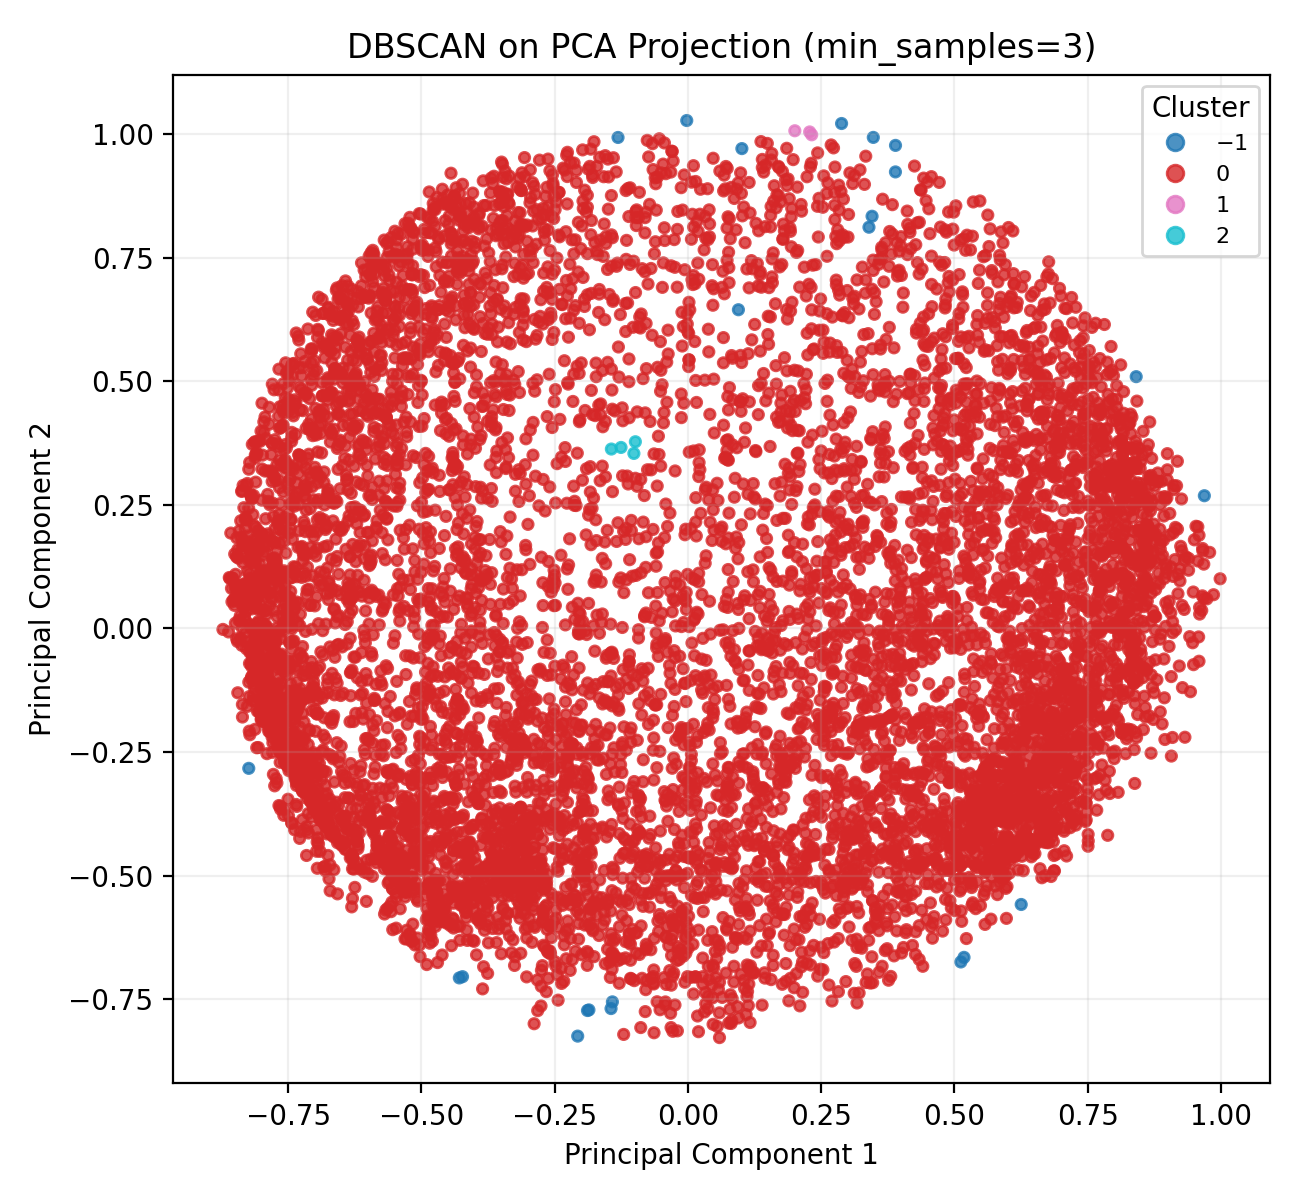
\includegraphics[width=\linewidth]{figures/pca_dbscan_min3.png}
    
    \vspace{0.3em}
    \centering \small \texttt{min\_samples = 3}

    \column{0.33\linewidth}
    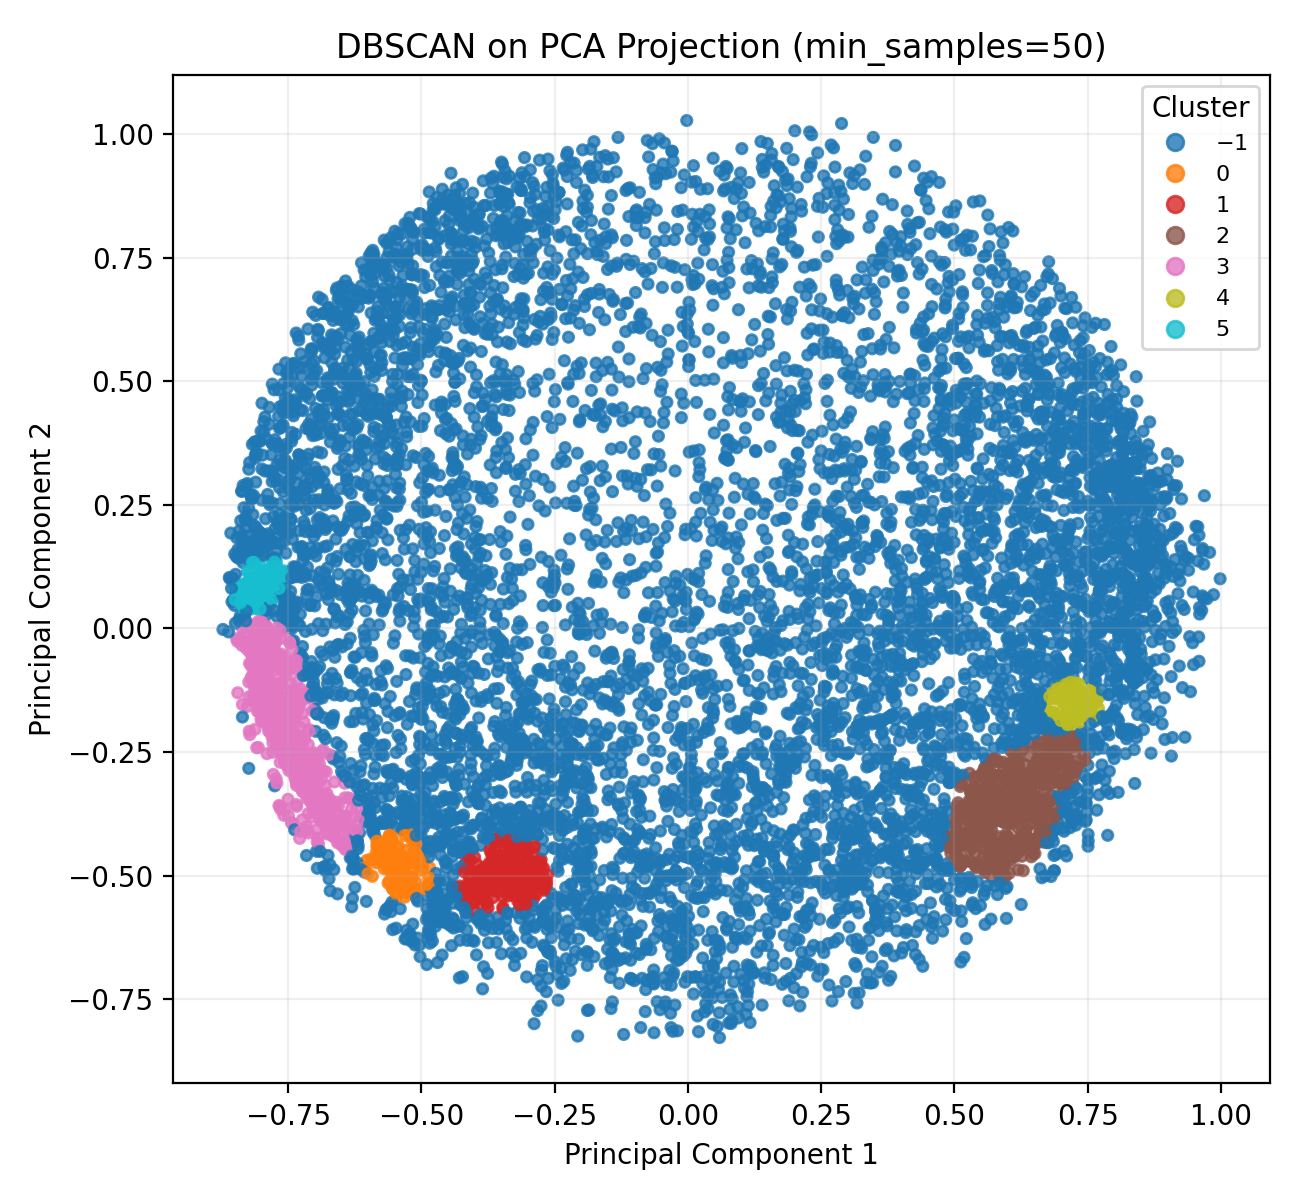
\includegraphics[width=\linewidth]{figures/pca_dbscan_min50.png}
    
    \vspace{0.3em}
    \centering \small \texttt{min\_samples = 50}

    \column{0.33\linewidth}
    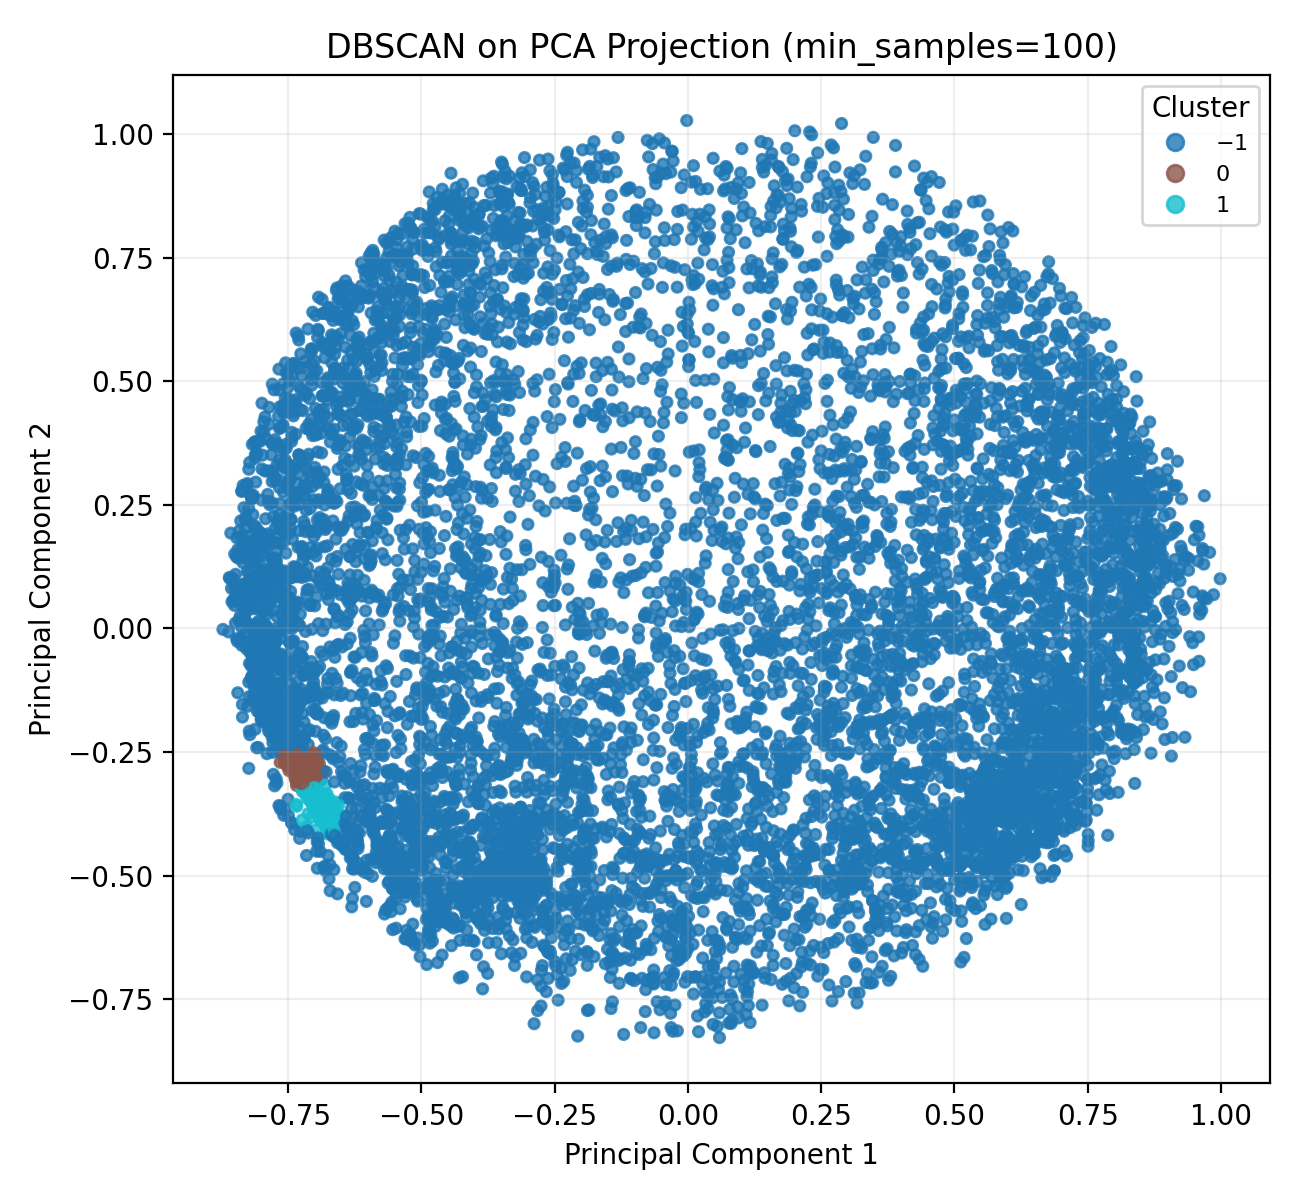
\includegraphics[width=\linewidth]{figures/pca_dbscan_min100.png}
    
    \vspace{0.3em}
    \centering \small \texttt{min\_samples = 100}
\end{columns}
\end{frame}

\begin{frame}{DBSCAN 해석 포인트}
\begin{itemize}
    \item \texttt{min\_samples=3}에서는 작은 밀도 집단도 군집으로 인정되기 쉽다.
    \item \texttt{min\_samples}를 키우면 더 조밀한 집단만 군집으로 남고, 많은 점이 노이즈로 밀려난다.
    \item 따라서 DBSCAN은 ``군집 수를 몇 개로 할까''보다 ``얼마나 촘촘해야 군집으로 볼까''를 묻는 알고리즘이다.
    \item 이 비교는 셀 \texttt{45--47}을 순서대로 실행하면서 보여주기 좋다.
\end{itemize}
\end{frame}

\begin{frame}{실습 전환 멘트: PCA + DBSCAN}
\begin{block}{슬라이드에서 노트북으로 넘어가는 순간}
\small
``이제 PCA가 데이터의 구조를 보이게 만들어 준 상태에서, DBSCAN의 \texttt{min\_samples} 값을 바꾸면 군집과 노이즈 해석이 어떻게 달라지는지 직접 보겠습니다. 노트북 셀 40번부터 47번까지가 바로 이 흐름입니다.''
\end{block}
\begin{block}{실행할 것}
\begin{itemize}
    \item \texttt{python\_3장.ipynb} 셀 \texttt{40--47}
    \item 비교 포인트: 전처리, PCA 2축 생성, DBSCAN 파라미터 변화
\end{itemize}
\end{block}
\end{frame}

\section{정리}
\begin{frame}{정리}
\begin{itemize}
    \item K-means는 군집 수를 먼저 정하고, 엘보우 곡선으로 적절한 \(k\)를 가늠한다.
    \item PCA는 고차원 데이터를 2차원으로 줄여 구조를 읽기 쉽게 만든다.
    \item DBSCAN은 군집 수를 미리 정하지 않고, 밀도에 따라 군집과 노이즈를 함께 판단한다.
    \item 이번 세미나는 교재 설명 후 곧바로 노트북 셀을 실행하는 방식으로 진행한다.
\end{itemize}
\end{frame}

\begin{frame}{노트북 체크리스트}
\begin{block}{K-means}
\begin{itemize}
    \item 셀 \texttt{34--39}
    \item 데이터 로드, 원-핫 인코딩, 정규화, 엘보우 곡선
\end{itemize}
\end{block}
\begin{block}{PCA + DBSCAN}
\begin{itemize}
    \item 셀 \texttt{40--47}
    \item 결측치 처리, 표준화, 정규화, PCA, DBSCAN 비교
\end{itemize}
\end{block}
\end{frame}

\end{document}
